\documentclass[]{IEEEphot}

\usepackage[style=numeric, backend=biber]{biblatex}  %biblatex
\addbibresource{Literatur.bib} %Datenbankdatei <-- Export aus Citavi im Latex Projekteordner
\usepackage[egnlish]{babel} % Silbentrennung
\usepackage[T1]{fontenc}      %z.B. für (besseres) automatisches Trennen nach Umlauten
\usepackage[section]{placeins} % Gleiten von Abbildungen verhindern
\usepackage{csquotes} %When using babel or polyglossia with biblatex, loading csquotes is recommended to
%ensure that quoted texts are typeset according to the rules of your main language.
\usepackage{hyperref}

\usepackage{graphicx}
\graphicspath{ {./Material/pictures/} }

\jvol{xx}
\jnum{xx}
\jmonth{Juni}
\pubyear{2021}

\newtheorem{theorem}{Theorem}
\newtheorem{lemma}{Lemma}

\begin{document}

	\title{Distance and movement measurement of an object based on stereo images}

	\author{Lennard Rose, Moritz Zeitler}

	\affil{Hochschule für angewandte Wissenschaften Würzburg-Schweinfurt\\
		Fakultät Informatik und Wirtschaftsinformatik}

	\maketitle

	\markboth{IEEE Photonics Journal}{Volume Extreme Ultraviolet Holographic Imaging}


	\begin{abstract}
		This paper explains how to compute distance to, and movement of an object within vision of a stereo camera.
		Included is the whole workflow consisting of all steps that have to be made to get such a recognition to work. These steps are the hardware setup, all calibration steps, object detection, object tracking and the measurements of the values themselves.
	\end{abstract}

	\section{Introduction}
	\label{sec:einfuehrung}
	From a high level standpoint the human eye is a very simple complex. It enables us to see things, even in color. But if we go deeper there is much more to our sight. For example we can see depth, which is very complex as a concept. This is based on the human eye having to different point-of-views. In this project the so called Stereo-Vision, will be translated to a computational level. To establish this we use a stereo camera setup to take photos/videos, create a depth map and try to compute the distance and movement of an object. The following chapters will describe this in a step by step fashion, starting with the theory behind it and the implementation afterwards.

	\section{Theoretical Basics}
	This chapter contains a detailed theoretical description of each individual step in the workflow.
	\subsection{Stereo Camera Calibration}
	Cameras are projecting a three dimensional object to a two dimensional image. This projection is never alone determined by the original object, but also by all parameters of the used camera. These you can separate in two groups, external and internal. External parameters are the camera orientation in different planes. Internal parameters are determined by the cameras internal characteristics.\newline
	\begin{figure}[h!]
	\centering
	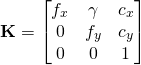
\includegraphics[scale=1]{intrinsicMatrix.png}
	\caption{Intrinsic Matrix}
	\end{figure}
	We can represent these internal parameters as an upper triangular matrix K. This matrix has the values fx and fy as the x and y focal lengths. cx and cy as the x and y coordinates of the optical center in the image plane. Gamma is the distortion between the axes, this value is replaced by a "0" in OpenCV´s calibration function.\newline
	\begin{figure}[h!]
		\centering
		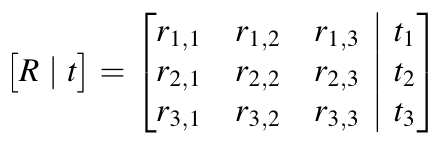
\includegraphics[scale=0.7]{extrinsicMatrix.png}
		\caption{Extrinsic Matrix}
	\end{figure}
	The external parameters are represented by an 3x3 rotation matrix, that indicates the rotation bias of the camera, combined with an 3x1 translation vector.\newline
	\begin{figure}[h!]
		\centering
		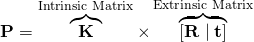
\includegraphics[scale=0.7]{projectionMatrix.png}
		\caption{Projection Matrix}
	\end{figure}
	Together these form the 3x4 Projection Matrix. This matrix and the 3D-coordinates of our point is used to calculate the image coordinates of the 2D projection. Calibration does nothing else than alter these matrices so our 2D projection matches the 3D object. This is usually done by giving the calibrating program/ function a set of 2D images with known 3D coordinates.\newline
	This Calibration consists of two steps removing of Distortion as well as rectifying the images.
	\subsubsection{Distortion}
	A camera lens always has some kind of curvature. This curvature is also visible in an image taken with this lens. This is called distortion. There are many different types of distortion which can be seen in the picture beneath.
	\begin{figure}[h!]
		\centering
		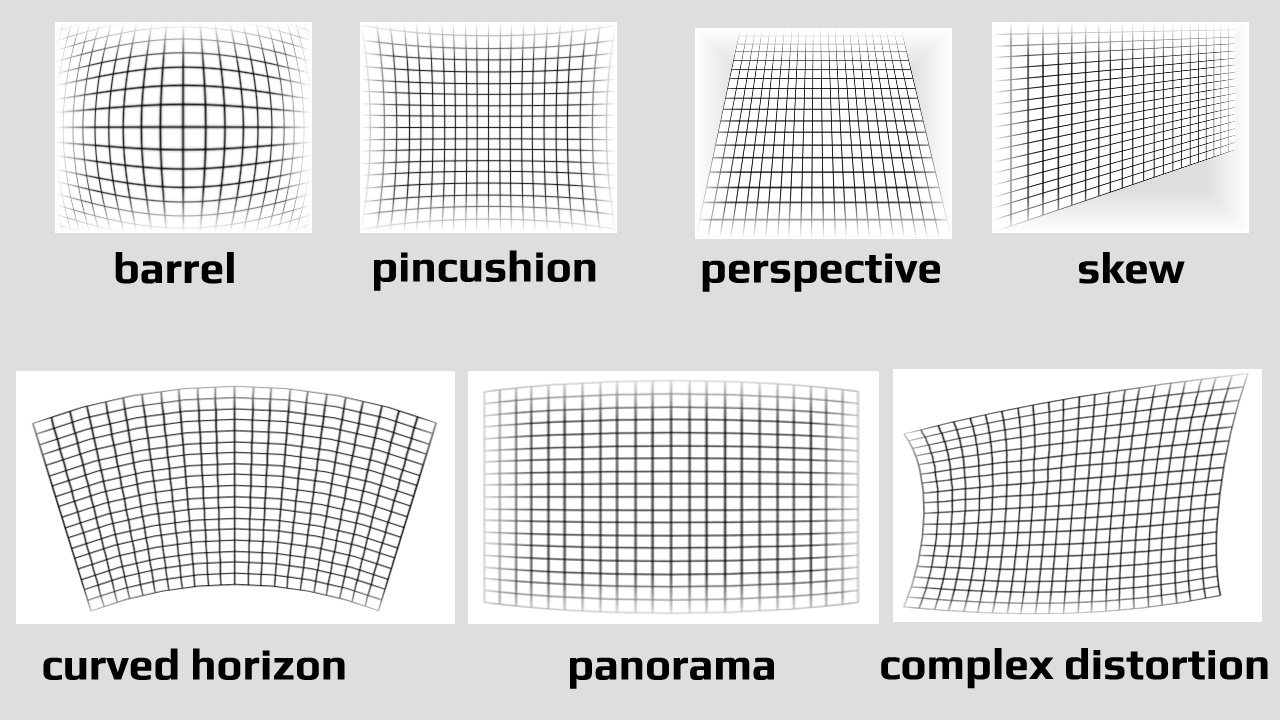
\includegraphics[scale=0.3]{distortion.jpg}
		\caption{Distortion types}
	\end{figure}
	To remove this distortion we take pictures of a chessboard. OpenCV, the package we use to do all calibration steps, can easily detect key points using this chessboard pattern. This is based on the big difference in pixel values between white and black. In combination with the size of the squares as well as the amount of the squares, OpenCV is able to create a calibration matrix removing the distortion.\newline
	A very important part is to be very precise while taking the calibration pictures. To get a good result you need to take calibration photos, basically of all parts of the pov of the camera.
	\subsubsection{Rectification}
	With image rectification, the goal is to map
	\subsection{Stereoscopy}
	\subsection{Disparity Map}
	\subsection{Depth Map}
	\subsection{Object Detection}
	\subsection{Object Tracking}
	\subsection{Measurements}
	\subsubsection{Distance}
	\subsection{Direction}
	\subsection{Speed}
	\section{Prerequisites}
	\section{Computation Pipeline}
	\section{Results}
	\section{Conclusion}

	\newpage

	\printbibliography[title={Literaturverzeichnis}]

\end{document}